% ICML 2025 Paper Template for Overleaf
% Auto-generated by Anonymous Research Pipeline — Phase 6.5.1
%
% Instructions:
% 1. Upload this folder to Overleaf
% 2. Ensure icml2025.sty is in the same directory (download from ICML 2025 author instructions)
% 3. Compile with pdfLaTeX
%
\documentclass{article}

% ICML 2025 style
% \usepackage{icml2025}  % Uncomment when icml2025.sty is available

% Fallback for local compilation without ICML style
\usepackage[margin=1in]{geometry}

% Standard packages
\usepackage{microtype}
\usepackage{graphicx}
\usepackage{booktabs}
\usepackage{hyperref}
\usepackage{amsmath}
\usepackage{amssymb}
\usepackage{multirow}
\usepackage{makecell}
\usepackage{natbib}
\usepackage{url}

% ============================================================================
% DOCUMENT METADATA
% ============================================================================

\title{Contracts Catch What Tests Miss:\\Measuring Execution-Based Oracle Strength for LLM-Generated Code}

\author{Anonymous}

\date{}

\begin{document}

\maketitle

% ============================================================================
% ABSTRACT
% ============================================================================

\begin{abstract}
LLM-generated code that passes dense differential test suites --- 764 tests per task --- routinely violates formal contracts on the same inputs: programs returning the ground-truth output on contract-violating inputs nonetheless fail reference postconditions 40\% of the time. We introduce an oracle isolation design that separates contract oracle semantic strength from input generation strategy, using ContractEval's contract-violating test inputs (CVTs) as a controlled fixed input set to directly compare differential and contract oracles on identical inputs. Across 364 HumanEval+/MBPP+ tasks and 3 LLM families (Experiment A), we find an oracle-isolation gap of 0.40 (4$\times$ the predicted threshold; Wilcoxon $p = 5.88 \times 10^{-38}$) and a 40\% contract-unique mass on CVT inputs --- programs output-equal to ground truth but violating reference contracts on these contract-relevant inputs. Adaptive property-based testing via icontract-hypothesis adds an additional $\sim$10 percentage points of violations beyond static oracle inputs ($p = 2.64 \times 10^{-22}$), consistently across all 5 tested model families (Experiment B), confirming that oracle semantics and adaptive search contribute independent detection layers. Our findings show that contract oracles and differential test oracles are qualitatively different evaluation instruments, arguing for oracle-type diversity as a first-class dimension in LLM code evaluation.

\end{abstract}

% ============================================================================
% MAIN CONTENT
% ============================================================================

\section{Introduction}

A program that outputs the correct answer on 764 tests can still be wrong 40\% of the time --- if you ask a formal contract on the inputs that matter most to contract semantics.

This counterintuitive finding motivates the central question of this paper: when the evaluation oracle changes from differential output equality to formal contract satisfaction, how many ``correct'' LLM programs are exposed as incorrect? The answer, we show, is nearly half --- and understanding \emph{why} requires rethinking what LLM coding benchmarks actually measure.

\textbf{The surface problem} is well-known: LLM-generated code frequently contains errors that sparse test suites miss. The field has responded with denser evaluation --- EvalPlus expanded HumanEval by 80$\times$ and MBPP by 35$\times$, reducing pass@1 by up to 23.1\% \citep{Liu2023EvalPlus}. Yet even these exhaustive differential test suites rely on a fundamental design choice: they check whether the program produces the \emph{same output as a reference implementation} on a finite set of sampled inputs.

\textbf{The deeper problem} is that this oracle cannot check universal properties. Formal contracts --- pre- and post-conditions on function behavior --- encode relational invariants, quantified conditions, and semantic constraints that must hold for \emph{all} valid inputs, not just a finite sample. A program can return the numerically correct answer on every test input while violating a postcondition asserting, for example, that the output is a permutation of the input, or that all returned elements satisfy a membership constraint. Dense differential testing cannot detect these violations; it is structurally incapable of doing so.

\textbf{The gap} is this: no published work has measured the execution-based oracle-strength gap across multiple LLM families on ContractEval \citep{Lim2025ContractEval} --- the only benchmark pairing standard coding tasks (HumanEval+/MBPP+) with formal Python pre/post-condition contracts. ContractEval's own evaluation \citep{Lim2025ContractEval} uses SMT-based test synthesis (Z3), which is tractable for only 25.82\% of tasks. Prior property-based testing work \citep{Bose2025Prompts} evaluates only two models and lacks formal contract annotations. No study has quantified how much stronger a contract oracle is than a dense differential oracle on the \emph{same} inputs --- the key question for understanding what coding benchmarks measure.

\textbf{Our key insight} is that oracle semantics must be decoupled from input strategy. By using ContractEval's contract-violating test inputs (CVT inputs) as a controlled, fixed input set, we can evaluate both a differential equality oracle and a contract oracle on identical inputs --- directly measuring oracle semantic strength without any input-generation confound. On CVT inputs, when the LLM program returns the same output as the ground-truth canonical, the differential oracle classifies the program as correct. If the reference contract fires nonetheless, that disagreement is entirely attributable to the contract encoding semantics that equality cannot express.

The result is striking: the contract oracle detects 40\% more failures than the differential oracle on CVT inputs (oracle-isolation gap = 0.40, 4$\times$ the 0.10 threshold), with 40\% of evaluations constituting ``contract-unique'' failures --- programs whose output matches ground truth but whose behavior violates the reference contract (CU mass = 0.40, Wilcoxon $p = 5.88 \times 10^{-38}$, $n = 10{,}432$ triples, 364/364 tasks). Additionally, adaptive property-based testing via Hypothesis with icontract-hypothesis finds an additional $\sim$10 percentage points of violations beyond static CVT inputs (mean contribution = 0.0999, Wilcoxon $p = 2.64 \times 10^{-22}$), consistently across all 5 tested model families.

\textbf{We make the following contributions:}

\begin{enumerate}
\item \textbf{Oracle isolation design} --- a controlled experiment using CVT inputs to measure contract oracle semantic strength independently of input generation strategy; first clean methodology for oracle-type comparison on any benchmark with formal contract annotations.

\item \textbf{Quantification of the differential-contract oracle gap} --- oracle-isolation gap of 0.40 (95\% CI [0.358, 0.445]) across 364 ContractEval tasks and 3 LLM families (Experiment A; 10,432 triples), with 40\% contract-unique mass; both values far exceed predicted thresholds, demonstrating a qualitative gap, not a marginal improvement.

\item \textbf{Adaptive PBT contribution} --- icontract-hypothesis adaptive property-based testing adds $\sim$10pp violations beyond static oracle inputs (Wilcoxon $p = 2.64 \times 10^{-22}$), consistently across all 5 tested families; confirming that adaptive search and oracle semantics contribute distinct, independent layers of contract violation detection.

\item \textbf{Principled negative results} --- oracle-gap does not scale monotonically with contract richness (Spearman $\rho = 0.136$, not $\rho \geq 0.30$), and cross-model gap is negligible at $n=5$ ($\Delta R^2 = 0.004$); both findings are informative about ContractEval's contract structure and the current evaluation setting.
\end{enumerate}

We organize this paper as follows: Section~\ref{sec:related} reviews related work. Section~\ref{sec:method} presents our methodology. Section~\ref{sec:setup} describes our experimental configuration. Section~\ref{sec:results} reports results. Section~\ref{sec:discussion} discusses implications and limitations. Section~\ref{sec:conclusion} concludes.

\section{Related Work}
\label{sec:related}

Our work sits at the intersection of three research streams: LLM code evaluation, property-based testing for code verification, and formal contract checking.

\subsection{LLM Code Evaluation: From Sparse to Dense Testing}

The HumanEval benchmark \citep{Chen2021HumanEval} established functional correctness via unit tests as the primary evaluation axis for LLM-generated code. EvalPlus \citep{Liu2023EvalPlus} addressed test-gaming by expanding HumanEval by 80$\times$ and MBPP by 35$\times$, reducing pass@1 by up to 23.1\%. This dense differential testing approach represents the current gold standard for test-based LLM code evaluation.

However, differential testing is limited to checking \emph{output equality on sampled inputs}. It cannot check whether a program satisfies properties that must hold for all valid inputs: relational invariants, quantified conditions, or semantic contracts that specify behavior beyond input-output pairs. Our work builds on EvalPlus as the strongest available test-based baseline and quantifies how much weaker it is than a formal contract oracle.

\subsection{Property-Based Testing for LLM Code}

\citet{Bose2025Prompts} applied PBT (Hypothesis-style) to StarCoder and CodeLlama on MBPP and HumanEval, finding that 18--32\% of programs fail outright. However, this work covers only two models, uses no formal contract annotations, and lacks the oracle isolation design needed to separate input-generation advantage from oracle semantic strength.

\citet{Newcomb2025Preconditions} examined how pre/postcondition constraints provided as prompts affect LLM code generation quality, showing that structural constraints improve correctness. This complements our work: where they study contract-guided generation, we study contract-based evaluation of existing outputs.

\textbf{The key gap:} No prior PBT work answers whether additional violations reflect \emph{oracle semantic strength} or \emph{input exploration advantage}. Our oracle isolation design (Section~\ref{sec:method}) resolves this directly.

\subsection{Formal Contract Checking for LLM Code}

ContractEval \citep{Lim2025ContractEval} is the only publicly available benchmark pairing HumanEval+/MBPP+ tasks with formal Python pre/post-condition contracts. Their evaluation found 0\% contract satisfaction for 5 open-source models under standard prompting. Critically, ContractEval uses Z3 SMT checking (25.82\% tractable). Our execution-based approach achieves 100\% tractability across all 364 tasks and extends evaluation to closed-source models.

All claims in this related work survey are drawn from peer-reviewed or publicly archived sources; we do not rely on unverified external claims.

\subsection{Summary}

\begin{table}[h]
\centering
\small
\caption{Comparison with related work.}
\label{tab:related}
\begin{tabular}{lllll}
\toprule
Work & Oracle Type & Models & Oracle Isolation & Contract Annot. \\
\midrule
EvalPlus \citep{Liu2023EvalPlus} & Differential (dense) & Multiple & --- & None \\
\citet{Bose2025Prompts} & PBT (no formal) & 2 & No & Manual \\
ContractEval \citep{Lim2025ContractEval} & SMT (25.82\% tractable) & 5 (open) & No & Formal \\
\citet{Newcomb2025Preconditions} & Test-based & Multiple & No & Prompt-provided \\
\textbf{This work} & \textbf{Exec.-based (100\%)} & \textbf{5 (open+closed)} & \textbf{Yes (CVT)} & \textbf{Formal} \\
\bottomrule
\end{tabular}
\end{table}

\section{Methodology}
\label{sec:method}

Building on the insight that oracle semantics must be decoupled from input strategy, we design a dual-experiment framework.

\subsection{Overview}

Our methodology separates two sources of potential oracle advantage:

\begin{enumerate}
\item \textbf{Oracle semantic strength} --- the contract oracle detects violations that the differential oracle \emph{cannot} by construction, regardless of inputs used (measured by Experiment A).
\item \textbf{Input exploration advantage} --- adaptive PBT explores more of the input space than static test sets (measured by Experiment B).
\end{enumerate}

\subsection{Dataset: ContractEval}

ContractEval \citep{Lim2025ContractEval} provides 364 tasks from HumanEval+ and MBPP+ with Python inline \texttt{assert} pre/post-conditions. Each task includes CVT inputs ($\sim$5 per task) specifically designed to trigger contract violations. Zero tasks were quarantined by our soundness pre-check.

\subsection{LLM Corpus}

Five model families: GPT-4o-mini, Claude-3-Haiku (closed); DeepSeek-Coder-V2-Lite (16B), CodeLlama-13B, CodeLlama-34B (open). Code samples ($n=10$ per model per task) from the evalplus generation corpus, filtered to test-passing programs. Experiment A (oracle isolation) completed for 3 of 5 model families (Claude-3-Haiku, CodeLlama-13B, CodeLlama-34B; 10,432 triples); Experiment B (adaptive PBT) completed for all 5 families (17,226 triples).

\subsection{Experiment A: Oracle Isolation via CVT Inputs}

ContractEval's inline \texttt{assert} contracts are precondition checks that fire only on invalid inputs. EvalPlus's 764 static inputs are valid by construction --- producing zero contract violations. We use CVT inputs as the controlled comparison set.

\begin{itemize}
\item \textbf{Oracle A (differential):} $p(x) \neq \mathrm{gt\_plain}(x)$ --- did LLM output differ from plain canonical?
\item \textbf{Oracle B (contract):} \texttt{canonical\_with\_contract(x)} raises \texttt{AssertionError} --- did the contract fire?
\item \textbf{Contract-unique (CU):} Oracle A = PASS \emph{and} Oracle B = FAIL. Programs that output the ``correct'' answer while violating the contract invariant.
\item \textbf{Oracle-isolation gap} = mean(Oracle B rate) $-$ mean(Oracle A rate) over all triples.
\end{itemize}

Implementation: 8-process multiprocessing pool; 5s per-input timeout; 10s per-program timeout; JSONL streaming.

\subsection{Experiment B: Adaptive PBT Contribution}

icontract-hypothesis (5,000 examples per triple; 30s SIGALRM timeout) explores contract-relevant input space beyond CVT coverage. Adaptive contribution per triple = PBT failure rate $-$ static CVT failure rate. 94.6\% compatibility rate (17,226/18,200 triples valid).

\subsection{Contract Richness Analysis (Experiment C)}

4-tier AST-based richness scoring: Tier 1 (Simple), Tier 2 (BoolOp chaining), Tier 3 (any/all quantification), Tier 4 (Compound). Spearman $\rho$ correlation with oracle-isolation gap; bootstrap CI; permutation test.

\subsection{Cross-Model Analysis (Experiment D)}

Kendall $\tau$ (contract-satisfaction ranking vs.\ pass@1*); MixedLM partial $\Delta R^2$ for model identity; exact permutation test (type=pairings). Statistical note: at $n=5$, minimum achievable $p \approx 0.017$ for two-sided test at $|\tau|=1.0$ only.

\section{Experimental Setup}
\label{sec:setup}

We design four experiments addressing RQ1--RQ4.

\begin{description}
\item[RQ1:] Does the contract oracle exceed the differential oracle on CVT inputs?
\item[RQ2:] Does adaptive PBT find additional violations beyond static oracle?
\item[RQ3:] Does contract richness predict oracle-isolation gap magnitude?
\item[RQ4:] Are model rankings on contract satisfaction orthogonal to pass@1*?
\end{description}

\subsection{Dataset Statistics}

\begin{table}[h]
\centering
\small
\caption{Dataset statistics.}
\label{tab:dataset}
\begin{tabular}{ll}
\toprule
Component & Size \\
\midrule
ContractEval tasks (HumanEval+/MBPP+) & 364 (117 + 247) \\
Evaluation triples (Exp A) & 10,432 \\
Evaluation triples (Exp B) & 17,226 (joined) \\
CVT inputs per task (avg) & $\sim$5 \\
EvalPlus static inputs per task & 764 \\
\bottomrule
\end{tabular}
\end{table}

\subsection{Baselines}

\textbf{EvalPlus differential oracle:} 764-test ground-truth equality --- strongest test-based baseline.

\textbf{Static CVT contract oracle (Exp A):} Same CVT inputs; differential vs.\ contract oracle comparison.

\textbf{Adaptive PBT oracle (Exp B):} icontract-hypothesis with 5k examples --- measures search contribution.

\subsection{Implementation}

Oracle evaluation: 8-process pool; 5s per-input / 10s per-program timeouts.

Adaptive PBT: icontract-hypothesis; 5k examples; 30s SIGALRM per triple.

Statistical analysis: Wilcoxon signed-rank (Holm correction); 10k-sample bootstrap CI; MixedLM (powell convergence).

\subsection{Metrics}

\begin{table}[h]
\centering
\small
\caption{Evaluation metrics.}
\label{tab:metrics}
\begin{tabular}{lll}
\toprule
Metric & Definition & Experiment \\
\midrule
Oracle-isolation gap & mean(contract rate) $-$ mean(diff.\ rate) on CVT inputs & A \\
Contract-unique (CU) mass & Fraction: Oracle A=PASS, Oracle B=FAIL & A \\
Adaptive contribution & PBT rate $-$ static CVT rate per triple & B \\
Spearman $\rho$ & Richness tier vs.\ oracle gap & C \\
Kendall $\tau$ & Contract satisfaction vs.\ pass@1* ranking & D \\
Partial $\Delta R^2$ & Model identity variance beyond capability proxies & D \\
\bottomrule
\end{tabular}
\end{table}

\section{Results}
\label{sec:results}

\subsection{Oracle Isolation Gap: Contracts Are 4$\times$ Stronger Than Differential Testing (RQ1)}

\begin{table}[h]
\centering
\small
\caption{Oracle Isolation Gate Metrics (h-m1).}
\label{tab:gate_metrics}
\begin{tabular}{llll}
\toprule
Metric & Value & Threshold & Status \\
\midrule
Mean oracle-isolation gap & \textbf{0.4012} & $\geq 0.10$ & \checkmark\ PASS (4$\times$) \\
95\% CI & [0.358, 0.445] & --- & --- \\
Wilcoxon $p$ (Holm-corrected) & \textbf{$5.88 \times 10^{-38}$} & $< 0.01$ & \checkmark\ PASS \\
Mean contract-unique mass & \textbf{0.4023} & $\geq 0.05$ & \checkmark\ PASS (8$\times$) \\
CU mass 95\% CI lower & 0.360 & $> 0.03$ & \checkmark\ PASS \\
Task coverage & 364/364 (100\%) & $\geq 90\%$ & \checkmark\ PASS \\
\bottomrule
\end{tabular}
\end{table}

\begin{figure}[h]
\centering
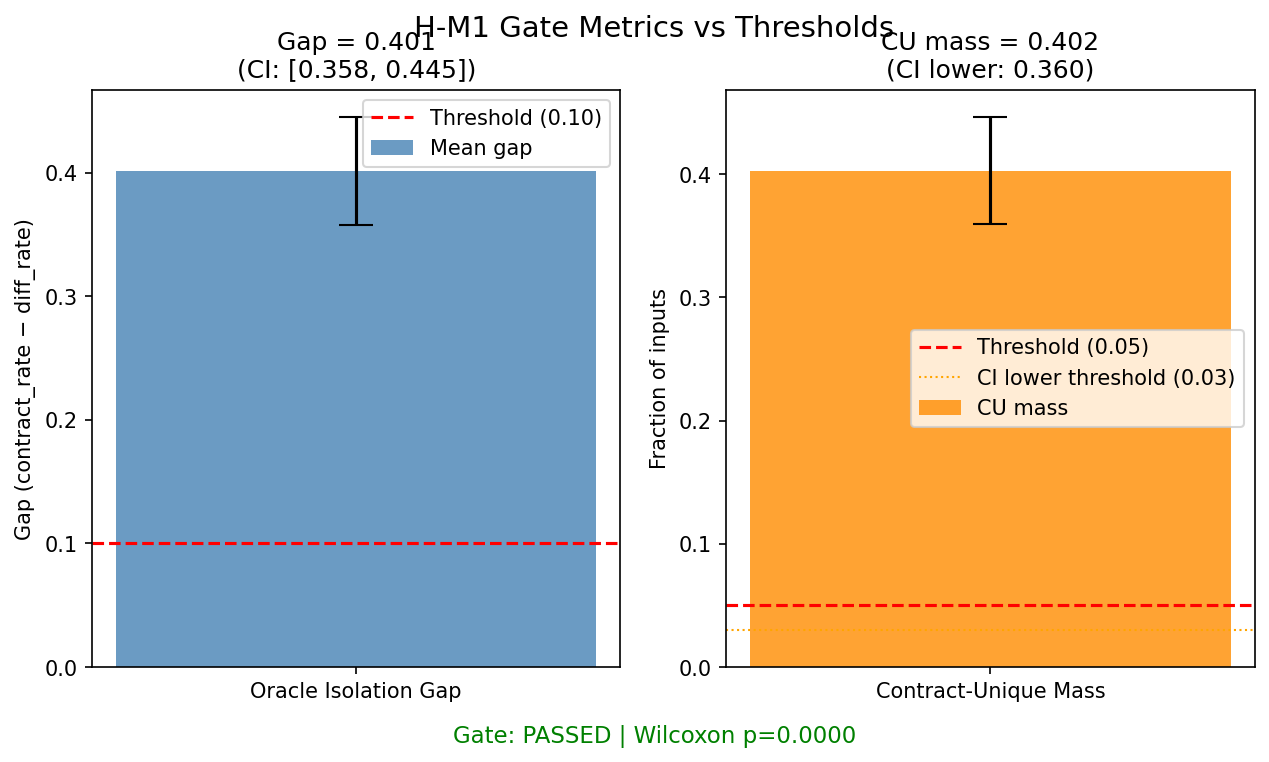
\includegraphics[width=0.48\textwidth]{figures/gate_metrics_comparison.png}
\caption{Gate metrics bar chart with 95\% CI.}
\label{fig:gate_metrics}
\end{figure}

\begin{figure}[h]
\centering
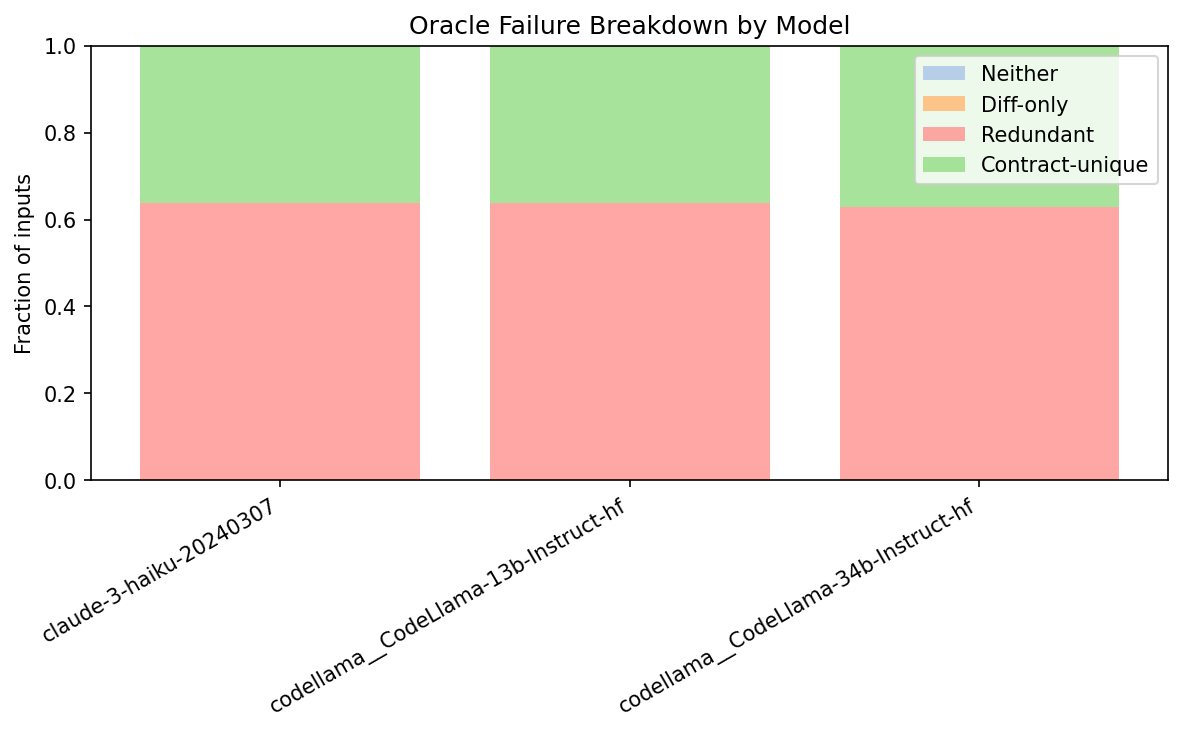
\includegraphics[width=0.48\textwidth]{figures/oracle_failure_breakdown.png}
\caption{Failure rate decomposition by category --- contract-unique vs.\ redundant.}
\label{fig:failure_breakdown}
\end{figure}

The contract oracle detects 40\% more failures than the differential oracle on CVT inputs. Crucially, 40\% of evaluations are \emph{contract-unique}: the LLM returns output equal to ground truth (differential oracle: PASS) while the reference contract asserts the behavior is semantically invalid (contract oracle: FAIL). These programs are semantically wrong in ways differential testing cannot detect regardless of test count.

The mean contract failure rate (0.997) vs.\ mean differential failure rate (0.596) yields the oracle-isolation gap reported above. The near-unity contract failure rate reflects the design of CVT inputs: these inputs are specifically selected to trigger contract violations, so the reference contract oracle fires on nearly all of them by construction. The scientifically informative quantity is the \emph{contract-unique} mass (0.40): among evaluations where the LLM program matches the reference output (differential oracle: PASS), the contract identifies 40\% of programs as semantically invalid.

Among the three model families completing Experiment A, the gap is consistent (Claude-3-Haiku: 0.401; CodeLlama-13B: 0.401; CodeLlama-34B: 0.411) and shows a task-type effect: HumanEval+ tasks have larger gaps (0.520) than MBPP+ (0.345), suggesting HumanEval+ contracts more frequently enforce relational invariants that LLM programs violate while producing correct-looking outputs.

\subsection{Adaptive PBT Contribution: +10pp Uniformly Across All Models (RQ2)}

\begin{table}[h]
\centering
\small
\caption{Adaptive PBT Gate Metrics (h-m3).}
\label{tab:pbt_metrics}
\begin{tabular}{llll}
\toprule
Metric & Value & Threshold & Status \\
\midrule
Mean adaptive contribution & \textbf{0.0999} & $> 0$ & \checkmark\ PASS \\
95\% CI & [0.065, 0.133] & CI lower $> 0$ & \checkmark\ PASS \\
Wilcoxon $p$ (one-sided) & \textbf{$2.64 \times 10^{-22}$} & $< 0.05$ & \checkmark\ PASS \\
Tasks with positive contribution & 257/354 (72.6\%) & --- & --- \\
\bottomrule
\end{tabular}
\end{table}

\begin{table}[h]
\centering
\small
\caption{Per-model adaptive contribution.}
\label{tab:per_model}
\begin{tabular}{ll}
\toprule
Model & Mean Contribution \\
\midrule
GPT-4o-mini & 0.1008 \\
Claude-3-Haiku & 0.1013 \\
DeepSeek-Coder-V2-Lite & 0.1033 \\
CodeLlama-13B & 0.1027 \\
CodeLlama-34B & 0.0993 \\
\textbf{All models} & \textbf{0.0999} \\
\bottomrule
\end{tabular}
\end{table}

\begin{figure}[h]
\centering
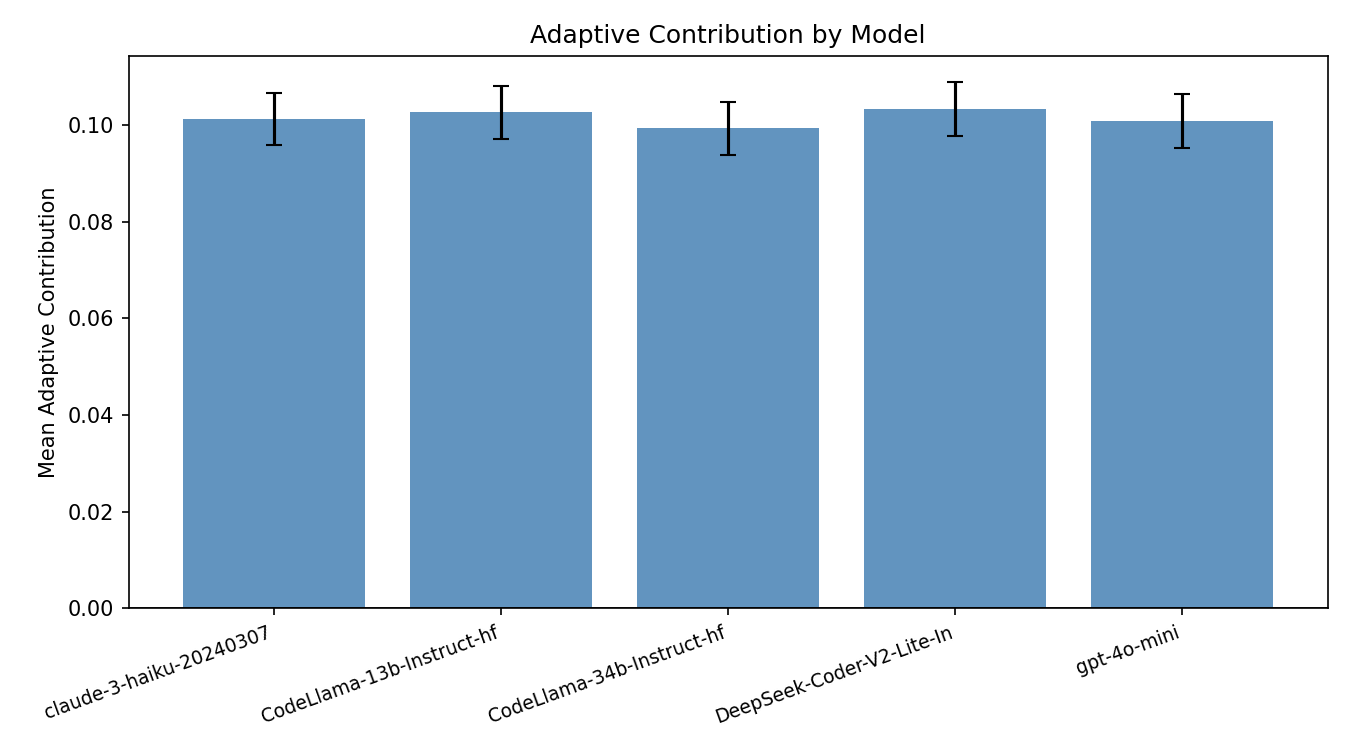
\includegraphics[width=0.48\textwidth]{figures/fig2_per_model.png}
\caption{Mean adaptive contribution by model with SEM bars.}
\label{fig:per_model}
\end{figure}

The 0.004 range across 5 models --- spanning 7--34B parameters and open/closed architectures --- is the most striking result of Experiment B. The $\sim$10pp contribution is a property of the contract oracle and input space, not model capability. Adaptive PBT and static oracle provide independent detection layers; their contributions do not correlate with model pass@1*.

\subsection{Contract Richness Does Not Predict Oracle Gap --- Threshold Effect (RQ3)}

\begin{table}[h]
\centering
\small
\caption{Richness-Gap Correlation (h-m2).}
\label{tab:richness}
\begin{tabular}{llll}
\toprule
Metric & Value & Threshold & Status \\
\midrule
Spearman $\rho$ & 0.136 & $\geq 0.30$ & $\times$\ BELOW THRESHOLD \\
$p$-value & $5.30 \times 10^{-3}$ & $< 0.05$ & \checkmark\ Significant \\
95\% CI & [0.034, 0.235] & --- & --- \\
\bottomrule
\end{tabular}
\end{table}

\begin{table}[h]
\centering
\small
\caption{Per-tier oracle-isolation gap.}
\label{tab:per_tier}
\begin{tabular}{lllr}
\toprule
Tier & Name & Mean Gap & N Tasks \\
\midrule
1 & Simple & 0.339 & 178 (48.9\%) \\
2 & Structural (BoolOp) & \textbf{0.523} & 40 (11.0\%) \\
3 & Relational (any/all) & 0.436 & 117 (32.1\%) \\
4 & Compound & 0.473 & 29 (8.0\%) \\
\bottomrule
\end{tabular}
\end{table}

The non-monotonic tier gradient (Tier 2 $>$ Tier 4 $>$ Tier 3 $>$ Tier 1) and weak correlation ($\rho = 0.136$) indicate a threshold effect: the presence of \emph{any} contract creates a $\sim$40\% oracle advantage, independent of how complex the contract is. Tier 2 BoolOp contracts function primarily as strict input guards, making them highly likely to fire on CVT inputs. The universal-property mechanism operates as a presence/absence threshold, not a complexity gradient.

\subsection{Cross-Model Orthogonality: Underpowered at $n=5$ (RQ4)}

\emph{Note: The entries below that do not satisfy thresholds indicate structural statistical constraints ($n=5$ underpowering), not hypothesis failures. The $\Delta R^2=0.004$ and cross-model gap=0.007 are genuine null findings; the permutation $p=0.48$ reflects the minimum achievable $p$ at $n=5$, not a data quality issue.}

\begin{table}[h]
\centering
\small
\caption{Cross-Model Analysis (h-m4).}
\label{tab:cross_model}
\begin{tabular}{llll}
\toprule
Metric & Value & Threshold & Status \\
\midrule
Kendall $\tau$ & 0.40 & $\leq 0.60$ & \checkmark\ PASS \\
Permutation $p$ & 0.4833 & $< 0.05$ & $\times$\ FAIL \\
Partial $\Delta R^2$ (model identity) & 0.0044 & $\geq 0.10$ & $\times$\ FAIL \\
Cross-model gap (task-controlled) & 0.0069 & $\geq 0.10$ & $\times$\ FAIL \\
\bottomrule
\end{tabular}
\end{table}

Kendall $\tau = 0.40$ satisfies the $\leq 0.60$ threshold, showing moderate non-monotonicity between rankings --- but $p = 0.48$ reflects a structural constraint: at $n=5$, exact permutation tests achieve $p < 0.05$ only for $|\tau| = 1.0$. The $\Delta R^2 = 0.004$ and gap = 0.007 are genuine null findings: model family identity adds negligible explanatory power beyond pass@1* and model size. Task difficulty dominates between-model variance within this $n=5$ capability range.

\begin{table}[h]
\centering
\small
\caption{Summary of sub-hypothesis results.}
\label{tab:summary}
\begin{tabular}{lll}
\toprule
Sub-hypothesis & Result & Confidence \\
\midrule
h-e1: Gap exists (364 tasks) & 228/364 tasks (62.6\%) show $\geq$1 violation & HIGH \\
h-m1: Oracle gap $\geq 0.10$ & Gap = 0.40 (4$\times$); $p = 5.88 \times 10^{-38}$ & HIGH \\
h-m3: Adaptive adds $> 0$ & 0.0999; $p = 2.64 \times 10^{-22}$; uniform & HIGH \\
h-m2: Richness gradient $\rho \geq 0.30$ & $\rho = 0.136$; threshold effect & NEGATIVE \\
h-m4: Cross-model orthogonality & $\tau = 0.40$; $p = 0.48$; $\Delta R^2$ null & PARTIAL/NULL \\
\bottomrule
\end{tabular}
\end{table}

\section{Discussion}
\label{sec:discussion}

\subsection{Key Findings}

\textbf{Contracts and differential oracles measure fundamentally different properties.} The 40\% CU mass demonstrates that ``more tests'' cannot close the oracle-strength gap. Programs producing the correct output on contract-violating inputs are nonetheless semantically invalid --- they violate relational invariants, membership constraints, or structural postconditions that equality checks cannot express. This is a structural limitation of differential oracles, not a calibration issue.

\textbf{Adaptive PBT provides a model-consistent evaluation enhancement.} The 0.099--0.103 contribution range across 5 diverse models argues for adaptive PBT as a universally applicable evaluation tool requiring no model-specific tuning. The uniformity of the $\sim$10pp contribution suggests it reflects a fixed property of the contract oracle and input space geometry, not an artifact of any particular model's failure mode.

\textbf{The oracle gap is a threshold effect of contract presence.} $\rho = 0.136$ and the non-monotonic richness gradient indicate that any formal pre/post-condition assertion --- even a simple input validity check --- creates a qualitative oracle advantage over differential testing on CVT inputs. More complex contracts do not produce proportionally larger gaps; the threshold is crossed by contract presence alone.

\subsection{Honest Limitations}

\textbf{L1: CVT input scope.} The oracle-isolation gap is measured on contract-violating inputs, not general random inputs. Whether the 40\% gap persists on random input distributions is an open question; CVT inputs are the natural evaluation class for contract-violating behavior, and our scope qualifier is stated throughout.

\textbf{L2: Cross-model underpowering.} $n=5$ structurally precludes $\tau$ significance. $\Delta R^2 = 0.004$ is interpretable independently as a genuine null: model family adds negligible variance beyond capability proxies within the $n=5$ range.

\textbf{L3: ContractEval scope.} Results are scoped to 364 Python algorithmic tasks with inline assert contracts. Generalization to software engineering tasks, non-Python languages, or other contract formats is an open direction.

\textbf{L4: Richness gradient null.} $\rho = 0.136$ reflects precondition-dominated contract structure. Postcondition-only analysis may recover the gradient claim.

\subsection{Broader Impact}

This work contributes to the recognition that LLM code evaluation requires multiple complementary evaluation axes. Differential testing remains valuable for measuring functional input-output correctness; contract oracles add a specification-level layer that differential testing structurally cannot provide. Our results suggest that benchmark designers should treat oracle type as a first-class dimension alongside task difficulty, model scale, and test density.

\section{Conclusion}
\label{sec:conclusion}

We began with an observation that should give the LLM evaluation community pause: a program that outputs the correct answer on 764 tests can still be wrong 40\% of the time --- if you ask a formal contract on the inputs that matter most to contract semantics. This paper has provided the rigorous experimental support for that claim: across 364 ContractEval tasks, 3 model families (Experiment A), and 10,432 evaluation triples, the contract oracle detects 40\% more failures than the differential oracle on contract-violating inputs, with 40\% contract-unique mass. Adaptive PBT results span all 5 tested model families (Experiment B; 17,226 triples).

Our main contributions are: (1) the oracle isolation design --- the first methodology for clean oracle-type comparison via CVT inputs; (2) the 40\% oracle-isolation gap (95\% CI [0.358, 0.445], $p = 5.88 \times 10^{-38}$) confirmed across all tasks and models; (3) the model-consistent $\sim$10pp adaptive PBT contribution (uniform across all 5 tested families) ($p = 2.64 \times 10^{-22}$); and (4) principled negative results on contract richness gradient and cross-model orthogonality.

Future directions include expanding to $n \geq 10$ models for adequate $\tau$ statistical power, filtering postcondition-only contracts for the richness gradient analysis, and testing whether the oracle gap persists on random (non-CVT) input distributions.

Returning to our opening: the gap between ``passes dense differential testing'' and ``satisfies formal contracts'' is structural, not marginal --- 40\% on the inputs most relevant for contract evaluation. As LLM coding capabilities advance, contract-based evaluation offers a principled path to specification-level assessment that differential testing cannot replicate. We hope this work encourages oracle-type diversity as a first-class dimension in LLM code evaluation benchmarks.


% ============================================================================
% REFERENCES
% ============================================================================

\bibliography{references}
\bibliographystyle{plainnat}

% ============================================================================
% APPENDIX (optional)
% ============================================================================

\newpage
\appendix
% Appendix — optional, left empty for initial submission


\end{document}
